\documentclass[a4wide,10pt]{article}
%\usepackage{a4wide}
\usepackage[applemac,utf8]{inputenc}
%\usepackage[danish]{babel}
\usepackage[T1]{fontenc}
\usepackage{pdfsync}
\usepackage{amsmath,amssymb,amsfonts} 
\usepackage[pdftex]{graphicx}
%\usepackage{wrapfig}
%\usepackage{color}
\usepackage[small,bf]{caption}

\begin{document}
\title{DSB Portfolio 2}
\author{Nis Sarup}
\date{\today}
\maketitle

\newpage

	\section{Fourier Transform method} % (fold)
	\label{sec:fourier_transform_method}
		Mathematica functions:
		\begin{eqnarray}
			t &=& 67; \nonumber \\
			m &=& \frac{t-1}{2}; \nonumber \\
			cH &:=& \frac{2\pi 1800}{8000}; \nonumber \\
			cL &:=& \frac{2\pi 800}{8000}; \nonumber \\
			h[0] &:=& \frac{cH-cL}{\pi}; \nonumber \\
			h[n\_] &:=& \frac{Sin[cH \cdot n]}{n\cdot \pi} - \frac{Sin[cL \cdot n]}{n\cdot \pi}; \nonumber \\
		\end{eqnarray}
		I get the results h[n] with n ranging from $-m$ to $m$:
		\begin{equation}
			Table[h[i], {i, -m, m, 1}] \nonumber
		\end{equation}
		This gives a large table of values which I copy into the MathLab program (Program 7.1 for example 7.3 in the book) and get the following graph:
		\begin{figure}[h]
			\centering
				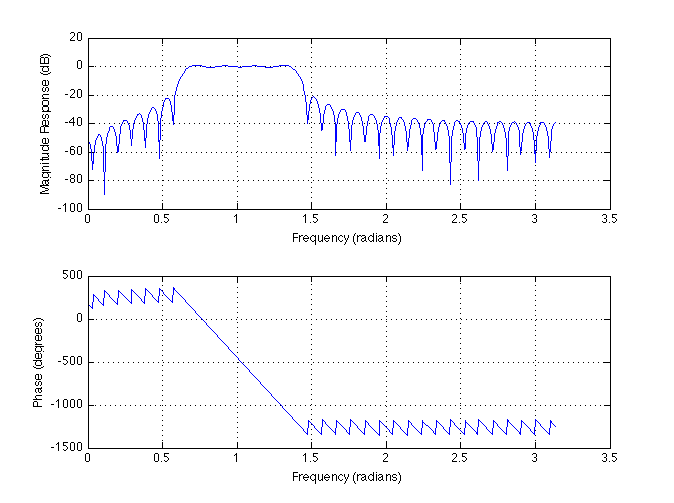
\includegraphics[width=9cm]{images/opgave_1.png}
			\caption{Fourier Transform method: Magnitude response and Phase.}
			\label{fig:images_opgave_1}
		\end{figure}
	% section fourier_transform_method (end)
	
	\newpage
	
	\section{Window Method} % (fold)
	\label{sec:window_method}
		\subsection{Rectangular Window} % (fold)
		\label{sub:rectangular_window}
			Mathematica function for the rectangular window:
			\begin{equation}
				rectangularWindow[n\_] := 1; \nonumber
			\end{equation}
			Not overly exciting. 
			For each value in the set from Section 1 I multiply it with the corresponding value from the window function. Here is a plot of the "new" graphs. 
			\begin{figure}[h]
				\centering
					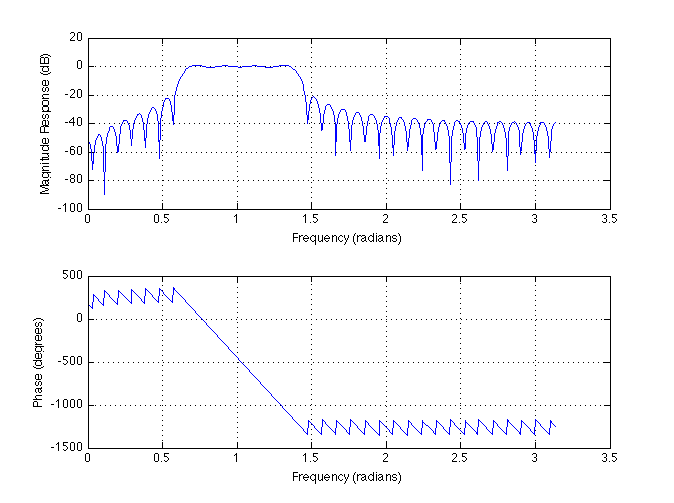
\includegraphics[width=9cm]{images/opgave_2_a.png}
				\caption{Rectangular window: Magnitude response and Phase.}
				\label{fig:images_opgave_2_a}
			\end{figure}
			Not surprisingly both Figure 1 and Figure 2 looks quite similar.
		% subsection rectangular_window (end)
		
\newpage		
		\subsection{Hamming Window} % (fold)
		\label{sub:hamming_window}
			Mathematica function for the Hamming Window:
			\begin{equation}
				hammingWindow[n\_] := 0.54 + 0.46 Cos[\frac{n\cdot \pi}{m}]; \nonumber
			\end{equation}
			Same procedure as with the Rectangular window. As can be seen there are some changes on this graph.
			\begin{figure}[h]
				\centering
					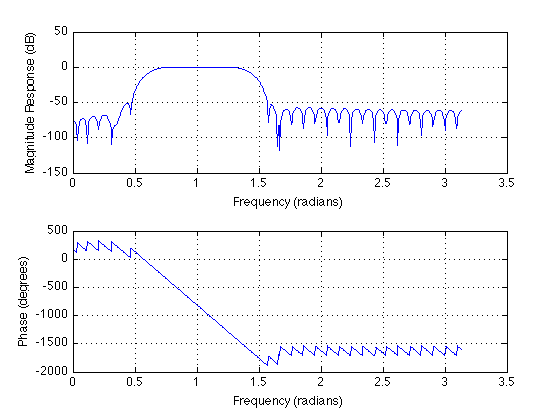
\includegraphics[width=9cm]{images/opgave_2_b.png}
				\caption{Hamming window: Magnitude response and Phase.}
				\label{fig:images_opgave_2_b}
			\end{figure}
			
		% subsection hamming_window (end)
		
\newpage
		\subsection{Kaiser Window} % (fold)
		\label{sub:kaiser_window}
		Mathlab has a build-in Kaiser-function, so I use that to generate the Kaiser window-values:
		\begin{eqnarray}
			beta &=& 0.5842*(50-21)^{0.4}+0.07886*(50-21); \nonumber \\
			wkaiser &=& kaiser(67, beta); \nonumber \\
		\end{eqnarray}
		THat particular equation for the Kaiser window is chosen because the specification calls for a stopband attenuation at 50dB.
		Again the values are multiplied and graphed.
		\begin{figure}[h]
			\centering
				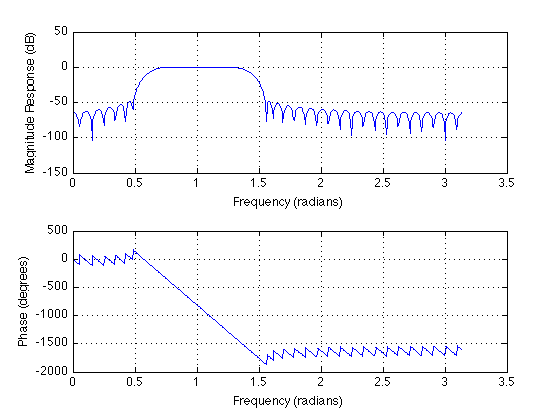
\includegraphics[width=9cm]{images/opgave_2_c.png}
			\caption{Kaiser window: Magnitude response and Phase.}
			\label{fig:images_opgave_2_c}
		\end{figure}
		
		% subsection kaiser_window (end)
	% section window_method (end)
	
\newpage
	\section{Frequency Sampling Method} % (fold)
	\label{sec:frequency_sampling_method}
		\subsection{Setup} % (fold)
		\label{sub:setup}
			I change the low cut frequency to 1000Hz and the upper cut frequency to 3000Hz. Here is the relevant mathematica functions ($cL$ and $cH$ is calculated the same way as in Section 1.):
			\begin{eqnarray}
				M &=& 12; \nonumber \\
				H[k\_] &:=& If[cL < \frac{2 \pi k}{2 M +1} < cH, 1, 0];  \nonumber \\
				h[n\_] &:=& \frac{1}{2M +1} (H[0] + 2 \sum\limits_{k=1}^M (H[k] Cos[\frac{2\pi k(n-M)}{2M+1}])); \nonumber \\
			\end{eqnarray}
			The bandpass frequency response vector is then:
			\begin{equation}
				\{0, 0, 0, 0, 1, 1, 1, 1, 1, 1, 0, 0, 0\} \nonumber \\
			\end{equation}
			And with a smooth transition:
			\begin{equation}
				\{0, 0, 0, 0.5, 1, 1, 1, 1, 1, 1, 0.5, 0, 0\} \nonumber \\
			\end{equation}
			Here is the plot for a 25 tap frequency sampling filter:
			\begin{figure}[h]
				\centering
					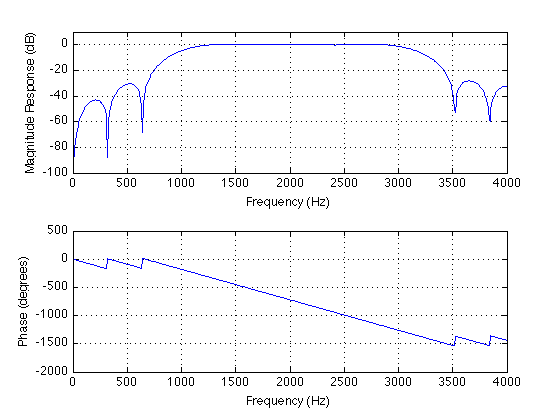
\includegraphics[width=9cm]{images/opgave_3_a_1.png}
				\caption{Frequency Sampling methos, with smooth transition.}
				\label{fig:images_opgave_3_a_1}
			\end{figure}
		% subsection setup (end)
\newpage
		\subsection{Increasing and decreasing the taps} % (fold)
		\label{sub:increasing_and_decreasing_the_taps}
		Increasing and decreasing the taps on a filter will have an effect. Here is plots of different tap sizes:
		\begin{figure}[h]
			\centering
				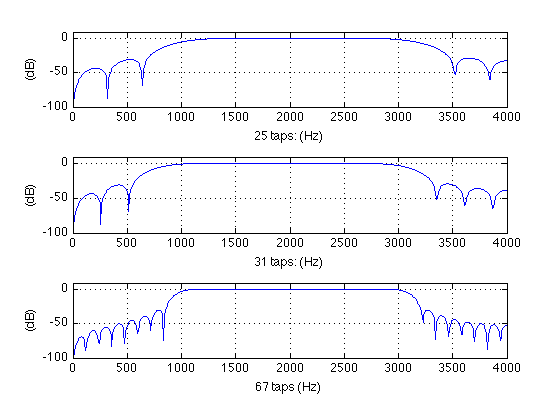
\includegraphics[width=9cm]{images/opgave_3_b.png}
			\caption{25, 31 and 67 tap Frequence Sampling filter plots.}
			\label{fig:images_opgave_3_b}
		\end{figure}
		% subsection increasing_and_decreasing_the_taps (end)
		\subsection{Discussion} % (fold)
		\label{sub:discussion}
			The higher the tap-number chosen when designing the Frequency Sampling filter, the higher the precision of the filter. The main-lobe follows a straight line better and dips faster at the cut-frequencies.
		% subsection discussion (end)
	% section frequency_sampling_method (end)
	
\newpage
	\section{Parks-McClellan algorithm} % (fold)
	\label{sec:parks_mcclellan_algorithm}
		Variables used:
		\begin{eqnarray}
			dP &=& 10^{\frac{0.05}{20}} -1 = 0,00577306 \nonumber \\
			dS &=& 10^{\frac{-50}{20}} = 0,00316228 \nonumber \\
			W &=& \frac{dP}{dS} = \frac{0,00577306}{0,00316228} \approx \frac{18}{10} \nonumber \\
			WS &=& 18 \nonumber \\
			WP &=& 10 \nonumber \\
		\end{eqnarray}
		The only things that needs changing from the MathLab program 7.16 in the book is the error weight factors and the order of the filter. The rest is the same. Here is the plot of the filter:
		\begin{figure}[h]
			\centering
				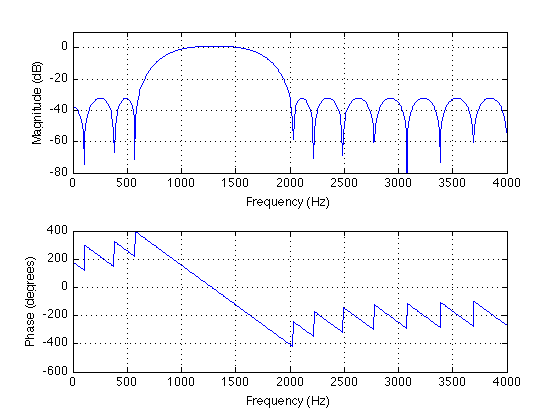
\includegraphics[width=9cm]{images/opgave_4.png}
			\caption{Parks-McClellan filter}
			\label{fig:images_opgave_4}
		\end{figure}
		I tried a few different orders to get the stopband attenuation below -50dB.
		
		Here is the MathLab code used:
		\begin{verbatim}
			fs = 8000;
			f = [0 0.15 0.25 0.4 0.5 1];
			m = [0 0 1 1 0 0];
			w = [18 10 18];
			format long
			b = remez(55,f,m,w)
			freqz(b,1,512,fs);
			axis([0 fs/2 -80 10])
		\end{verbatim}
	% section parks_mcclellan_algorithm (end)
\newpage
	\section{Discussion of the four design methods} % (fold)
	\label{sec:discussion_of_the_four_design_methods}
		\subsection{Fourier and Windowed Fourier Transform Method} % (fold)
		\label{sub:fourier_and_windowed_fourier_transform_method}
			I'll discuss the Normal and windowed Fourier Transform Methods as one here as they are quite similar.
			\begin{itemize}
				\item Somewhat simple.
				\item Can be done on a calculator if needed.
				\item Can only be used for lowpass, highpasss, stopband and passband filters.
			\end{itemize}
		% subsection fourier_and_windowed_fourier_transform_method (end)
		
		\subsection{Discussion of the Frequency Sampling method} % (fold)
		\label{sub:discussion_of_the_frequency_sampling_method}
			\begin{itemize}
				\item Simple equations.
				\item Can also be done on a calculator.
				\item Can be used for arbitrary filters, not only the 4 common types.
			\end{itemize}
		% subsection discussion_of_the_frequency_sampling_method (end)
		
		\subsection{Discussion of Parks-McClellan method} % (fold)
		\label{sub:discussion_of_parks_mcclellan_method}
			\begin{itemize}
				\item Complicated equations.
				\item A computer is needed.
				\item Can also be used to design arbitrary filters.
			\end{itemize}
		% subsection discussion_of_parks_mcclellan_method (end)
	Having the computational power available, I would probably use the last method.
	% section discussion_of_the_four_design_methods (end)
\end{document}